%%
%% This work is distributed under the LaTeX Project Public License (LPPL)
%% ( http://www.latex-project.org/ ) version 1.3, and may be freely used,
%% distributed and modified. A copy of the LPPL, version 1.3, is included
%% in the base LaTeX documentation of all distributions of LaTeX released
%% 2003/12/01 or later.
%% Retain all contribution notices and credits.
%% ** Modified files should be clearly indicated as such, including  **
%% ** renaming them and changing author support contact information. **
%%*************************************************************************



\documentclass[journal,transmag]{IEEEtran}

% *** MISC UTILITY PACKAGES ***
%
%\usepackage{ifpdf}
% Heiko Oberdiek's ifpdf.sty is very useful if you need conditional
% compilation based on whether the output is pdf or dvi.
% usage:
% \ifpdf
%   % pdf code
% \else
%   % dvi code
% \fi
% The latest version of ifpdf.sty can be obtained from:
% http://www.ctan.org/pkg/ifpdf
% Also, note that IEEEtran.cls V1.7 and later provides a builtin
% \ifCLASSINFOpdf conditional that works the same way.
% When switching from latex to pdflatex and vice-versa, the compiler may
% have to be run twice to clear warning/error messages.






% *** CITATION PACKAGES ***
%
%\usepackage{cite}
% cite.sty was written by Donald Arseneau
% V1.6 and later of IEEEtran pre-defines the format of the cite.sty package
% \cite{} output to follow that of the IEEE. Loading the cite package will
% result in citation numbers being automatically sorted and properly
% "compressed/ranged". e.g., [1], [9], [2], [7], [5], [6] without using
% cite.sty will become [1], [2], [5]--[7], [9] using cite.sty. cite.sty's
% \cite will automatically add leading space, if needed. Use cite.sty's
% noadjust option (cite.sty V3.8 and later) if you want to turn this off
% such as if a citation ever needs to be enclosed in parenthesis.
% cite.sty is already installed on most LaTeX systems. Be sure and use
% version 5.0 (2009-03-20) and later if using hyperref.sty.
% The latest version can be obtained at:
% http://www.ctan.org/pkg/cite
% The documentation is contained in the cite.sty file itself.






% *** GRAPHICS RELATED PACKAGES ***
%
\ifCLASSINFOpdf
  % \usepackage[pdftex]{graphicx}
  % declare the path(s) where your graphic files are
  % \graphicspath{{../pdf/}{../jpeg/}}
  % and their extensions so you won't have to specify these with
  % every instance of \includegraphics
  % \DeclareGraphicsExtensions{.pdf,.jpeg,.png}
\else
  % or other class option (dvipsone, dvipdf, if not using dvips). graphicx
  % will default to the driver specified in the system graphics.cfg if no
  % driver is specified.
  %\usepackage[dvips]{graphicx}
  % declare the path(s) where your graphic files are
  %\graphicspath{{../img/}}
  % and their extensions so you won't have to specify these with
  % every instance of \includegraphics
  % \DeclareGraphicsExtensions{.eps}
\fi
% graphicx was written by David Carlisle and Sebastian Rahtz. It is
% required if you want graphics, photos, etc. graphicx.sty is already
% installed on most LaTeX systems. The latest version and documentation
% can be obtained at: 
% http://www.ctan.org/pkg/graphicx
% Another good source of documentation is "Using Imported Graphics in
% LaTeX2e" by Keith Reckdahl which can be found at:
% http://www.ctan.org/pkg/epslatex
%
% latex, and pdflatex in dvi mode, support graphics in encapsulated
% postscript (.eps) format. pdflatex in pdf mode supports graphics
% in .pdf, .jpeg, .png and .mps (metapost) formats. Users should ensure
% that all non-photo figures use a vector format (.eps, .pdf, .mps) and
% not a bitmapped formats (.jpeg, .png). The IEEE frowns on bitmapped formats
% which can result in "jaggedy"/blurry rendering of lines and letters as
% well as large increases in file sizes.
%
% You can find documentation about the pdfTeX application at:
% http://www.tug.org/applications/pdftex




% *** MATH PACKAGES ***
%
%\usepackage{amsmath}
% A popular package from the American Mathematical Society that provides
% many useful and powerful commands for dealing with mathematics.
%
% Note that the amsmath package sets \interdisplaylinepenalty to 10000
% thus preventing page breaks from occurring within multiline equations. Use:
%\interdisplaylinepenalty=2500
% after loading amsmath to restore such page breaks as IEEEtran.cls normally
% does. amsmath.sty is already installed on most LaTeX systems. The latest
% version and documentation can be obtained at:
% http://www.ctan.org/pkg/amsmath





% *** SPECIALIZED LIST PACKAGES ***
%
%\usepackage{algorithmic}
% algorithmic.sty was written by Peter Williams and Rogerio Brito.
% This package provides an algorithmic environment fo describing algorithms.
% You can use the algorithmic environment in-text or within a figure
% environment to provide for a floating algorithm. Do NOT use the algorithm
% floating environment provided by algorithm.sty (by the same authors) or
% algorithm2e.sty (by Christophe Fiorio) as the IEEE does not use dedicated
% algorithm float types and packages that provide these will not provide
% correct IEEE style captions. The latest version and documentation of
% algorithmic.sty can be obtained at:
% http://www.ctan.org/pkg/algorithms
% Also of interest may be the (relatively newer and more customizable)
% algorithmicx.sty package by Szasz Janos:
% http://www.ctan.org/pkg/algorithmicx




% *** ALIGNMENT PACKAGES ***
%
%\usepackage{array}
% Frank Mittelbach's and David Carlisle's array.sty patches and improves
% the standard LaTeX2e array and tabular environments to provide better
% appearance and additional user controls. As the default LaTeX2e table
% generation code is lacking to the point of almost being broken with
% respect to the quality of the end results, all users are strongly
% advised to use an enhanced (at the very least that provided by array.sty)
% set of table tools. array.sty is already installed on most systems. The
% latest version and documentation can be obtained at:
% http://www.ctan.org/pkg/array


% IEEEtran contains the IEEEeqnarray family of commands that can be used to
% generate multiline equations as well as matrices, tables, etc., of high
% quality.




% *** SUBFIGURE PACKAGES ***
%\ifCLASSOPTIONcompsoc
%  \usepackage[caption=false,font=normalsize,labelfont=sf,textfont=sf]{subfig}
%\else
%  \usepackage[caption=false,font=footnotesize]{subfig}
%\fi
% subfig.sty, written by Steven Douglas Cochran, is the modern replacement
% for subfigure.sty, the latter of which is no longer maintained and is
% incompatible with some LaTeX packages including fixltx2e. However,
% subfig.sty requires and automatically loads Axel Sommerfeldt's caption.sty
% which will override IEEEtran.cls' handling of captions and this will result
% in non-IEEE style figure/table captions. To prevent this problem, be sure
% and invoke subfig.sty's "caption=false" package option (available since
% subfig.sty version 1.3, 2005/06/28) as this is will preserve IEEEtran.cls
% handling of captions.
% Note that the Computer Society format requires a larger sans serif font
% than the serif footnote size font used in traditional IEEE formatting
% and thus the need to invoke different subfig.sty package options depending
% on whether compsoc mode has been enabled.
%
% The latest version and documentation of subfig.sty can be obtained at:
% http://www.ctan.org/pkg/subfig



% *** FLOAT PACKAGES ***
%
%\usepackage{fixltx2e}
% fixltx2e, the successor to the earlier fix2col.sty, was written by
% Frank Mittelbach and David Carlisle. This package corrects a few problems
% in the LaTeX2e kernel, the most notable of which is that in current
% LaTeX2e releases, the ordering of single and double column floats is not
% guaranteed to be preserved. Thus, an unpatched LaTeX2e can allow a
% single column figure to be placed prior to an earlier double column
% figure.
% Be aware that LaTeX2e kernels dated 2015 and later have fixltx2e.sty's
% corrections already built into the system in which case a warning will
% be issued if an attempt is made to load fixltx2e.sty as it is no longer
% needed.
% The latest version and documentation can be found at:
% http://www.ctan.org/pkg/fixltx2e


%\usepackage{stfloats}
% stfloats.sty was written by Sigitas Tolusis. This package gives LaTeX2e
% the ability to do double column floats at the bottom of the page as well
% as the top. (e.g., "\begin{figure*}[!b]" is not normally possible in
% LaTeX2e). It also provides a command:
%\fnbelowfloat
% to enable the placement of footnotes below bottom floats (the standard
% LaTeX2e kernel puts them above bottom floats). This is an invasive package
% which rewrites many portions of the LaTeX2e float routines. It may not work
% with other packages that modify the LaTeX2e float routines. The latest
% version and documentation can be obtained at:
% http://www.ctan.org/pkg/stfloats
% Do not use the stfloats baselinefloat ability as the IEEE does not allow
% \baselineskip to stretch. Authors submitting work to the IEEE should note
% that the IEEE rarely uses double column equations and that authors should try
% to avoid such use. Do not be tempted to use the cuted.sty or midfloat.sty
% packages (also by Sigitas Tolusis) as the IEEE does not format its papers in
% such ways.
% Do not attempt to use stfloats with fixltx2e as they are incompatible.
% Instead, use Morten Hogholm'a dblfloatfix which combines the features
% of both fixltx2e and stfloats:
%
% \usepackage{dblfloatfix}
% The latest version can be found at:
% http://www.ctan.org/pkg/dblfloatfix




%\ifCLASSOPTIONcaptionsoff
%  \usepackage[nomarkers]{endfloat}
% \let\MYoriglatexcaption\caption
% \renewcommand{\caption}[2][\relax]{\MYoriglatexcaption[#2]{#2}}
%\fi
% endfloat.sty was written by James Darrell McCauley, Jeff Goldberg and 
% Axel Sommerfeldt. This package may be useful when used in conjunction with 
% IEEEtran.cls'  captionsoff option. Some IEEE journals/societies require that
% submissions have lists of figures/tables at the end of the paper and that
% figures/tables without any captions are placed on a page by themselves at
% the end of the document. If needed, the draftcls IEEEtran class option or
% \CLASSINPUTbaselinestretch interface can be used to increase the line
% spacing as well. Be sure and use the nomarkers option of endfloat to
% prevent endfloat from "marking" where the figures would have been placed
% in the text. The two hack lines of code above are a slight modification of
% that suggested by in the endfloat docs (section 8.4.1) to ensure that
% the full captions always appear in the list of figures/tables - even if
% the user used the short optional argument of \caption[]{}.
% IEEE papers do not typically make use of \caption[]'s optional argument,
% so this should not be an issue. A similar trick can be used to disable
% captions of packages such as subfig.sty that lack options to turn off
% the subcaptions:
% For subfig.sty:
% \let\MYorigsubfloat\subfloat
% \renewcommand{\subfloat}[2][\relax]{\MYorigsubfloat[]{#2}}
% However, the above trick will not work if both optional arguments of
% the \subfloat command are used. Furthermore, there needs to be a
% description of each subfigure *somewhere* and endfloat does not add
% subfigure captions to its list of figures. Thus, the best approach is to
% avoid the use of subfigure captions (many IEEE journals avoid them anyway)
% and instead reference/explain all the subfigures within the main caption.
% The latest version of endfloat.sty and its documentation can obtained at:
% http://www.ctan.org/pkg/endfloat
%
% The IEEEtran \ifCLASSOPTIONcaptionsoff conditional can also be used
% later in the document, say, to conditionally put the References on a 
% page by themselves.




% *** PDF, URL AND HYPERLINK PACKAGES ***
%
\usepackage{url}
% url.sty was written by Donald Arseneau. It provides better support for
% handling and breaking URLs. url.sty is already installed on most LaTeX
% systems. The latest version and documentation can be obtained at:
% http://www.ctan.org/pkg/url
% Basically, \url{my_url_here}.

\usepackage{graphicx}
\usepackage{multirow}



% *** Do not adjust lengths that control margins, column widths, etc. ***
% *** Do not use packages that alter fonts (such as pslatex).         ***
% There should be no need to do such things with IEEEtran.cls V1.6 and later.
% (Unless specifically asked to do so by the journal or conference you plan
% to submit to, of course. )


% correct bad hyphenation here
\hyphenation{op-tical net-works semi-conduc-tor}


\begin{document}
%
% paper title
% Titles are generally capitalized except for words such as a, an, and, as,
% at, but, by, for, in, nor, of, on, or, the, to and up, which are usually
% not capitalized unless they are the first or last word of the title.
% Linebreaks \\ can be used within to get better formatting as desired.
% Do not put math or special symbols in the title.
\title{\textsc{Why not engineering?} A study on the influence of gender factors on student's higher education choice.}



% author names and affiliations
% transmag papers use the long conference author name format.

\author{\IEEEauthorblockN{Paloma de las Cuevas\IEEEauthorrefmark{1}, and
Maribel Garc\'{i}a-Arenas\IEEEauthorrefmark{1}}
\IEEEauthorblockA{\IEEEauthorrefmark{1}Department of Computer Architecture and Computer Technology, ETSIIT and CITIC. University of Granada, Granada, Spain.}% <-this % stops an unwanted space
\thanks{Corresponding author: P. de las Cuevas (email: palomacd@ugr.es).}}



% The paper headers
%\markboth{Journal of \LaTeX\ Class Files,~Vol.~14, No.~8, August~2015}%
%{Shell \MakeLowercase{\textit{et al.}}: Bare Demo of IEEEtran.cls for IEEE Transactions on Magnetics Journals}
% The only time the second header will appear is for the odd numbered pages
% after the title page when using the twoside option.
% 
% *** Note that you probably will NOT want to include the author's ***
% *** name in the headers of peer review papers.                   ***
% You can use \ifCLASSOPTIONpeerreview for conditional compilation here if
% you desire.




% If you want to put a publisher's ID mark on the page you can do it like
% this:
%\IEEEpubid{0000--0000/00\$00.00~\copyright~2015 IEEE}
% Remember, if you use this you must call \IEEEpubidadjcol in the second
% column for its text to clear the IEEEpubid mark.



% use for special paper notices
%\IEEEspecialpapernotice{(Invited Paper)}


% for Transactions on Magnetics papers, we must declare the abstract and
% index terms PRIOR to the title within the \IEEEtitleabstractindextext
% IEEEtran command as these need to go into the title area created by
% \maketitle.
% As a general rule, do not put math, special symbols or citations
% in the abstract or keywords.
\IEEEtitleabstractindextext{%
\begin{abstract}
The fact that universities have been experimenting a decreasing tendency for women to study engineering poses a problem, because Europe, as well as the States, keep demanding for the best engineers to continue developing innovative products. This problem, thus, can be solved by answering the following question, which is what we try to do in this paper, how do we make STEM (Science, Technology, Engineering, and Mathematics) subjects more attractive to girls and teenager women?
There is a need to make this distinction between girls and boys because we have found that the factors that influence them for not studying an engineering are not always the same. This means that there are some influence factors in common, such as the environment, their view about themselves, and their knowledge about engineerings; however, the existing stereotypes about engineers mostly affect girls.
In this work we present the results of an analysis on the influence factors, and more precisely, the influence of gender factors, affecting student's higher education choice, particularly engineering. Moreover, we have observed and identified the influence of these factors in a High School in Granada (Spain), where we have conducted a survey among the students of different educational levels. % De lo de educational levels no estoy muy segura.
\end{abstract}

% Note that keywords are not normally used for peerreview papers.
\begin{IEEEkeywords}
Keyword, keyword.
\end{IEEEkeywords}}



% make the title area
\maketitle


% To allow for easy dual compilation without having to reenter the
% abstract/keywords data, the \IEEEtitleabstractindextext text will
% not be used in maketitle, but will appear (i.e., to be "transported")
% here as \IEEEdisplaynontitleabstractindextext when the compsoc 
% or transmag modes are not selected <OR> if conference mode is selected 
% - because all conference papers position the abstract like regular
% papers do.
\IEEEdisplaynontitleabstractindextext
% \IEEEdisplaynontitleabstractindextext has no effect when using
% compsoc or transmag under a non-conference mode.







% For peer review papers, you can put extra information on the cover
% page as needed:
% \ifCLASSOPTIONpeerreview
% \begin{center} \bfseries EDICS Category: 3-BBND \end{center}
% \fi
%
% For peerreview papers, this IEEEtran command inserts a page break and
% creates the second title. It will be ignored for other modes.
\IEEEpeerreviewmaketitle

\section{Introduction}
\label{sec:intro}

\IEEEPARstart{C}{onsidering} the increasing need of researchers and engineers in Europe \cite{gago2004europe}, European governments have mobilised in order to try making the students more interested in engineering \cite{Kearney2014}. In addition, the OECD\footnote{Organisation for Economic Co-operation and Development} showed in \cite{OECD2006} that less than 40\% of the students in science and engineering related careers are women. More particularly and recent, a study by The Institution of Engineering and Technology in UK, have found that only 17.4\% of computer science undergraduates, and 15.8\% of engineering and technology undergraduates are women \cite{IET::stats}. The same happens in Spain, where this number falls from the European mean to 31\%, taking into account all engineerings (civil, computer science, technology, and aeronautics, among others). Actually, the change in the higher education system, named ``the Bologna Process'' in Spain \cite{wagenaar2008universities} did not improve this situation, but the tendency in women enrollment in technology related degrees continue falling to 25\% (Data source: \cite{datos::uni}.).

On the other hand, EEUU is experiencing a similar situation. The National Center for Women \& Information Technology released a report in 2012 \cite{NCWIT::stats} where they reveal that 18\% of all students in computer and information sciences degrees are girls although girls represent the 57\% of all students of undergraduate degrees.

Given these statistics, and the fact that they are similar all over the world, it is crucial that we understand why this is happening, as in the near future the demand for engineers will be even higher. 

In this work we try to clarify if the influence factors found in the literature are valid for a High School in Granada (Spain), where a series of surveys have been conducted to students from different educational levels, even vocational technical education students. To this end, the paper is structured as follows. First, the influence factors to be studied are identified in Section \ref{sec:factores}, where an extensive review of the literature and existing surveys have generated a list of factors which equally affect boys and girls, and other affecting girls mostly. Then, in Section \ref{sec:EdA} we review the existing solutions that try to balance the ratio men-women in technology related degrees. The context in which the surveys have been carried out is detailed in Section \ref{sec:metodologia}, where the reasons to use those precise questions are explained and supported by literature. Finally, in Section \ref{sec:resultados} we discuss the obtained results, not only in general but also depending on the course level, so that in Section \ref{sec:conclusiones} we conclude the discussion about influence factors and set the foundation to answer the question ``how do we make STEM subjects more attractive to girls and teenager women?''.

\section{Factors of influence on student's higher education choice}
\label{sec:factores}

When identifying the influence factors that affect children and teenagers in chosing their higher education or degrees, we are interested not only in those that have an effect in general, but also gender factors. We have looked for different studies performed in EEUU, Europe, and Spain particularly, because the surveyed students for our results are boys and girls from an Spanish high school.

A variety of conclusions about the things that influence teenagers into choosing one degree or anothes can be found in \cite{everis2012}, which is a study carried out in Catalonia (Spain) to students in the last courses of high school. Thus, not taking into account the results by gender, the authors have found that:

\begin{itemize}
	\item Students who succeed in STEM\footnote{Science, Technology, Engineering, and Mathematics} subjects, have a tendency to continue with technology related studies, and have more probability of choosing an engineering degree. On the contrary, those that are not very good at STEM normally choose other degrees.
	\item In general, less than 33\% of science track in high school claim to be sure that they will continue their studies in an engineering degree.
	\item In both secondary and high school, students choose to study engineering depending on how capable they see themselves. This fact is more recognisable on girls, who tend to underestimate themselves. Hence, girls do not normally think about not choosing engineerings due to their difficulty, but because they think that they are not skilled enough to do it.
	\item Students' interest in new technologies, such as smartphones, tablets, or smartwatches, are not decisive in the final choice of studying an engineering degree.
	\item Altough in a lesser way than their perception about their own capabilities, their view, positive or negative, about the career prospects and the engineers themselves is an important part in their final decision.
\end{itemize}

When asked about stereotypes, the authors do not found that the students think about the engineers as ``geeks'' in a bad sense, however, they did observe a sexist perception of engineerings. This way, up to 60\% of the surveyed students think that engineering degrees are ``for men'', while only 42\% marked that they are also ``for women''. Actually, when separating the results by gender, they found that in Secondary School, the difference between boys and girls wanting to study an engineering is of 14\%, and grows to 31\% in High School. Also, the socioeconomic position of the families make these percentages even more acute, meaning that girls coming from families with high income have more probability to study an engineering degree than one with lower income.

In view of these results, there is a need to further study the gender factors that might influence students when choosing a degree. Particularly for this work, we want to find why there are so few women in engineering. For this reason, a European Project called ``Mind the Gap'' has been analysed. In a deliverable of this project \cite{mtg2015} the researchers compare the situation of women in technology in three different countries, the Netherlands, United Kingdom, and Spain.
There are some similarities, such as the fact that the girls' environment is very influential, being their families the most. Furthermore, the concept of ``family'' itself is a decisive factor, as the researchers observed that the interviewees percieved that long workdays do not reconcile with ``their housewife tasks''.

Another factor they observed in common in the three analysed countries was how unconfident the girls felt with STEM subjects or engineerings, because they are crowded with men, and that was an uncomfortable environment for them. On the other hand, teachers represent another influential factor, because they do not know how to cope with stopping the continuation of stereotypes, although they admit is happening. The results of the deliverable of ``Mind the Gap'' can be also found in the vast majority of the literature. To cite a few, in \cite{hill2010so} the AAUW\footnote{American Association of University Women} tried to identify the reasons whay there were so few women in STEM degrees or careers, concluding that the main factors are: the continuation of the old belief that women are worse than men at mathematics, even if nowadays this has been proven wrong; the general assumption of women not being interested in technology; and in the scope of STEM companies, family reconciliation.

Finally, a study of 2013 \cite{hazari2013factors} is worth mentioning, because some of the questions used in their interviews have been included in the surveys made for this paper, described in Section \ref{sec:metodologia}. In this study, Hazari et al. try to demonstrate how various actions can be opposing factors to those identified as negative. This way, the authors also asked the students about their interest in engineerings, and at the same time, about the representation of women among their classmates and teachers, and if there has been any activity in their schools that implied talking about the underrepresentation of women in STEM. The last was the only activity they could relate to a change of opinion in girls, from negative to positive, about the interest for STEM or engineering degrees.

In the following Section we are going to present some initiatives that try to overcome the negative factors that have been presented, and look for a growth in the interest of girls for engineering.

\section{State of the Art}
\label{sec:EdA}

Following the results summarised in Section \ref{sec:intro}, and taking into account the statements from \cite{everis2012}, to which they conclude that the interest for engineerings can be increased by activities that cover the needs of the underrepresented collectives. In the case of this work, the underrepresented group we are focusing on are women, and thus we describe in this Section the activities, initiatives, communities, and projects that try to encourage women in studying engineering. All analysed proposals have this same purpose, but can be classified depending on their way to achieve it.

\subsection{Research projects}

Funded by the European Union, the governments, or the universities themselves, aiming to go deeply into the reasons why women continue being unerrepresented in STEM and engineering or technology. Usually, the result of these research projects is a number of actions to take in order to respond to identified needs. However, if these actions are finally implemented, it is done by the time the project has finished and no more fundings are available.

An example of these projects is the aforementioned ``Mind the Gap'' \cite{mtg:site}, which has been partly funded by the European Erasmus+ program. Their aims are mainly two:

\begin{itemize}
  \item Helping teachers to make girls more interested in STEM subjects.
  \item To motivate girls so that they gain enough self-confidence to study STEM degrees, which for them is a mostly-male world.
\end{itemize}

To this end, they have defined three activities:

\begin{itemize}
  \item Formative courses for STEM teachers, so that they are provided with the necessary knowledge and tools to achieve the first aim.
  \item Periodical meetings with girls who show or feel self-confidence problems when thinking about studying STEM degrees. These meetings are called ``Career circles'' and are focused in students or teachers in different ways:
  \begin{itemize}
    \item In the meetings with the girls, a woman mentor supports and guides them towards getting over their lack of self-confidence. In addition, they help the girl students in enforcing the needed abilities to get on in an engineer environment, which now is mainly populated by men.
    \item The meetings with STEM teachers are more focused in talking about what problems women have to face in technology, how can they help them when they are still at school or high school, and sharing teaching methodologies.
  \end{itemize}
  \item Create an LMS (Learning Management System) such as Moodle, that is free and gathers all material that has been created during the proyects.
\end{itemize}

\subsection{Groups and communities}

These are non-profit girl groups or ``clubs'' who are interested in technology and periodically gather to talk about technology or discuss about the situation of women in STEM. As they are non-profitable organisations, whenever they need resources such as places to gather or material, they can be sponsored by companies.

Since women started getting rights such as the right to study at the University, the right to vote, or to work \cite{glover1995women}, a lot of women associations have appeared. It is the case of the aforementioned AAUW, that was founded in 1881 for University women. Also, it is now common that the governments include gender equality inside their ministries or offices, as it happens with Spain \cite{inmujer:site}, UK \cite{ukgequ:site}, and USA \cite{uswomen:site, aauw:site}, to cite a few.

In addition, there are more recent, their number constantly growing, groups, communities, or ``clubs'', dedicated to different activities related to encouraging women into STEM. In \cite{kira2012} there is a list of the most important organisations, classified by the specific purpose: encourage women in technology, share job offers, and share knowledge about programming, among other categories.

\begin{itemize}
	\item Study groups, that share basic knowledge about technology with girls and women, in order to make them feel that they are capable of studying an engineering or work in anything related to STEM, and stop thinking that it ``is not for them (women)''. These groups can also be used by women already studying or working with something STEM-related. There are both paying and free courses, sometimes even funded by companies or famous people \cite{karliek2012}.
	\item Local groups by city, such as the ``Girls in Tech'' coummunity \cite{git:site}, founded in 2007 and with headquarters in 54 cities all over the world, including Africa, Asia, Australia, Europe, Middle East, North America, and South America. They share job offers and organise conferences, activities, courses, and camps.
	\item Communities, media, and events, that try to inspire, mentor, and share ideas with women interested in STEM.
	\item Investors or accelerators, who mostly invest in new companies founded by women, or have women as executives.
	\item Professional organisations and alliances, where ``Women in Technology'', similar to ``Girls in Tech'', is mentioned.
	\item Groups, communities, or associations that organise activities and talks for little girls and teenagers, in order to ease the effects caused by the different influence factors (see Section \ref{sec:factores}) that makes them not to study anything STEM related.
\end{itemize}

\subsection{Code camps, campus, and occasional activities}

They are similar to the activities organised in groups or communities, but made non-periodically. Even if they are somehow periodical, for instance every year, they last a short period of time and look for a specific aim which is not to form an active community. Nonetheless, they can also be funded or sponsored by companies. 

The same way as with the organisations and groups, each year new code camps are offered, sometimes by those mentioned organisations, and because of the demanding for engineers as said in Section \ref{cap1:intro}. Many are for both boys and girls, others for girls only, paid or free, and some are celebrated in summer. In \cite{lauren2015} the author gathers many options that are intended for girls only, and the duration in time is variable. In Spain, for instance, most of the camps are mixed, as in \cite{cmadrid:site} and \cite{cbcn:site}, accepting boys and girls from 4-5 to 17 years old. In these kind of camps, students learn robotics, making videogames, programming, and making of smartphone applications. que admiten chicos y chicas entre 4 o 5 y 17 años. En ellos, se hacen actividades de robótica, programación de videojuegos y de aplicaciones tipo ``apps''. Both  \cite{cmadrid:site} and \cite{cbcn:site} where contacted in order to know the ratio among boys and girls but there was no response.

However, we could access the enrolment data from similar summer camps held at the University of Granada. These two camps are celebrated one a year, and last two weeks. The first one \cite{cinfant:site} is for kids, no matter the gender, from 7 to 13 years old. Sources from the organisation report that only 30\% of the students every year are girls. To this end, this University also holds a girls summer camp \cite{cchicas:site}, from 14 to 18 years old. Campuses that are only for girls helps creating a confident environment, which is key to encourage them into learning STEM, as has been demonstrated in Section \ref{sec:factores}. Sources of the University also report that many of the girls participating in this campus have ended studying an engineering degree.

\section{Methodology}
\label{sec:metodologia}

In order to check wether the factors analysed in Section \ref{sec:factores} are valid or not, a proper context must be found, so that results from the performed surveys can be compared with what has been foun in the literature. Therefore, in the search for a high school where to perform the analysis, we have studied the context of the different places from different points of view that are now described.

\subsection{Socio-economic environment}

It is important to know what is the socio-economic status of the students and their families, given that in Section \ref{sec:factores} it has been stated that the wealth of the families influences in the education of the children, and so it influences in the election of a certain degree, or to continue the studies at all.

The neighborhood in which the school is situated, is the second more habitated in Granada (South of Spain), and holds both the traditionally workers neighborhood face, and a more modern and wealthy one, due to the placement of the Astrophysics Center or the main hospital of the city.

\subsection{The centre}

The resources of the studied centre are also influential, since a good equipment in subjects such as Computer Science or Technology makes easier to engage children into STEM degrees.

In this way, the center, called ``Zaid\'{i}n-Vergeles'' \cite{iesZV:2013}, has 7.000 $m^2$ of extension with open and closed spaces. This high school opens during the whole day, because there are classes in the morning, and also during the afternoon. The courses available at Zaid\'{i}n-Vergeles are the whole secondary education, and vocational courses (see Appendix \ref{ap:courses} for more clarification about the educational system in Spain). As such, surveyed alumni are from a variety of age and social condition, mainly medium class. In addition, there is an active \textit{parents association} that promotes gender equality and colaborative initiatives, such as displays or conferences.

The chosen high school has an ICT (Information and Communication Technologies) classroom for the upper secondary education courses. It has 23 computers, which makes the students to work in pairs. Although, in every normal classroom, there is at least one computer, placed on the teacher's table. The students of the vocational courses have access to classrooms with enough computers for each one, but some bring their own. Furthermore, there are laptops available to all teachers who request them, so that they can carry special or interactive activities in their classes.

\subsection{The student body}

Knowing the students is key for knowing the global status of the school before chosing the sample. The global sdistribution of students per course are displayed in Table \ref{tab:alumni}. In this table, it is necessary to distinguish between students from the technical courses. Therefore, inside the upper secondary courses, approximately the 50\% are studying ``science'' - which includes both technological and medical specialities -, and almost the 31\% are in ``computer science'' or ``technology'' related vocational courses.

\begin{table*}
  \caption[Students per course at the surveyed high school]{Distribution of students per course and year at ``Zaid\'{i}n-Vergeles'', the high school where the surveys were performed. Approximate age is also indicated.}
  \label{tab:alumni}

  \begin{center}
    \begin{tabular}{|c|c|c|c|}
    	\hline
    	\multirow{3}{*}{Course} & \multicolumn{3}{l|}{Number of students \& Aprox. Age}  \\ \cline{2-4} 
    	& 2015-2016 & 2016-2017 & Age \\ \hline
    	``E.S.O.''(Compulsory secondary education), years 3 and 4 & 243 & & 12 - 18 \\ \hline
    	``Bachillerato''(Upper secondary education)    			  & 185 & & 16 - 20 \\ \hline
    	``Ciclos Formativos''(Vocational courses)      			  & 802 & & 18 -  \\ \hline
    \end{tabular}
  \end{center}
\end{table*}

\subsection{Academics}

In some way, the teachers are also related to the resources, or can be considered resources themselves. In addition, it is of interest to this study the analysis of the ratio between female and male STEM teachers, so that it can be studied if the students have STEM women as role models. At the studied high schoool, the ratio between men and women, in the departments we are interested in, is described if Table \ref{tab:teachers}.

\begin{table*}
	\caption[Teachers in STEM departments]{Distribution of gender among the teachers from deparments related to STEM.}
	\label{tab:teachers}
	
	\begin{center}
		\begin{tabular}{|c|c|c|}
			\hline
			\textbf{Department} & \textbf{Male Teachers} & \textbf{Female Teachers} \\ \hline
			Science & 3 & 2 \\ \hline
			Computer Science & 20 & 8 \\ \hline
			Mathematics & 6 & 2 \\ \hline
			Technology & 0 & 3 \\
			\hline
		\end{tabular}
	\end{center}
\end{table*}


The students undertook the survey while they where at class, and the classes visited where always related to Technology or Computer science. The courses range from the last of high school to technical courses for undergraduates. In addition, the surveys were carried on two different academic years, 2015-2016 and 2016-2017, to ensure a bigger sample. The total amount of students and the distribution is detailed in Table \ref{tab:muestra}.

\begin{table*}
  \caption[Students who undertook the surveys]{Distribution of students per course where the survey was undertaken.}
  \label{tab:muestra}

  \begin{center}
    \begin{tabular}{|c|c|c|c|c|}
    	\hline
    	\multirow{3}{*}{Course} & \multicolumn{4}{l|}{Number of students \& Gender distribution}  \\ \cline{2-5} 
    	& \multicolumn{2}{l|}{2015-2016} & \multicolumn{2}{l|}{2016-2017} \\ \cline{2-5} 
    	& Male & Female & Male & Female \\ \hline
    	Compulsory secondary education, years 3 and 4 & 33 & 30 & 12 & 25 \\ \hline
    	Upper secondary education, both years         & 26 & 10 & 52 & 45 \\ \hline
    	Vocational courses                            & 46 & 4 & 189 & 15 \\ \hline
    \end{tabular}
  \end{center}
\end{table*}

Following the indications given in \cite{cohen2013research}, the questions and answers of the research have been built taking into account that:

\begin{itemize}
  \item 
\end{itemize}

Therefore, the surveys have a total of 15 questions, and are available online as they have been created with the Google Forms tool \footnote{\url{https:\\drive.google.com}}. There are three different surveys; one for the compulsory secondary education courses, another for the upper secondary education courses, and the third one for the vocational courses. Although, all of them have the same head and introduction - briefly explaining the purpose of the survey -, and the questions are mostly alike, but there are particular differences in the answers when asking about their future plans. There are three types of questions: multiple choice, numeric scale, and multiple selection. Inside the multiple choice ones, they can be presented in a simple way, meaning that there is a question and two or more answer, one of which the student has to choose; or in the form of a table, where the rows are different but related questions and the colums represent the answers, being these either a sentence, a word, or a number.

In the next Section we will analyse the results globally, but worth mentioning cases will also be commented.

\section{Results}
\label{sec:results}

The tool used to create the surveys offers a graphic summary of the responses, however, as in some cases we would like to observe the comparison between courses, a processing of the raw data is mandatory. Therefore, and to start with, the distribution of boys and girls who have been surveyed per course is depicted in Figure \ref{fig:alumni}. It can be observed that the percentage of female students quickly falls as the course level grow, being less than 10\% in the vocational courses, the same found in science degrees as presented in Section \ref{sec:intro}.

\begin{figure}
  \centering
  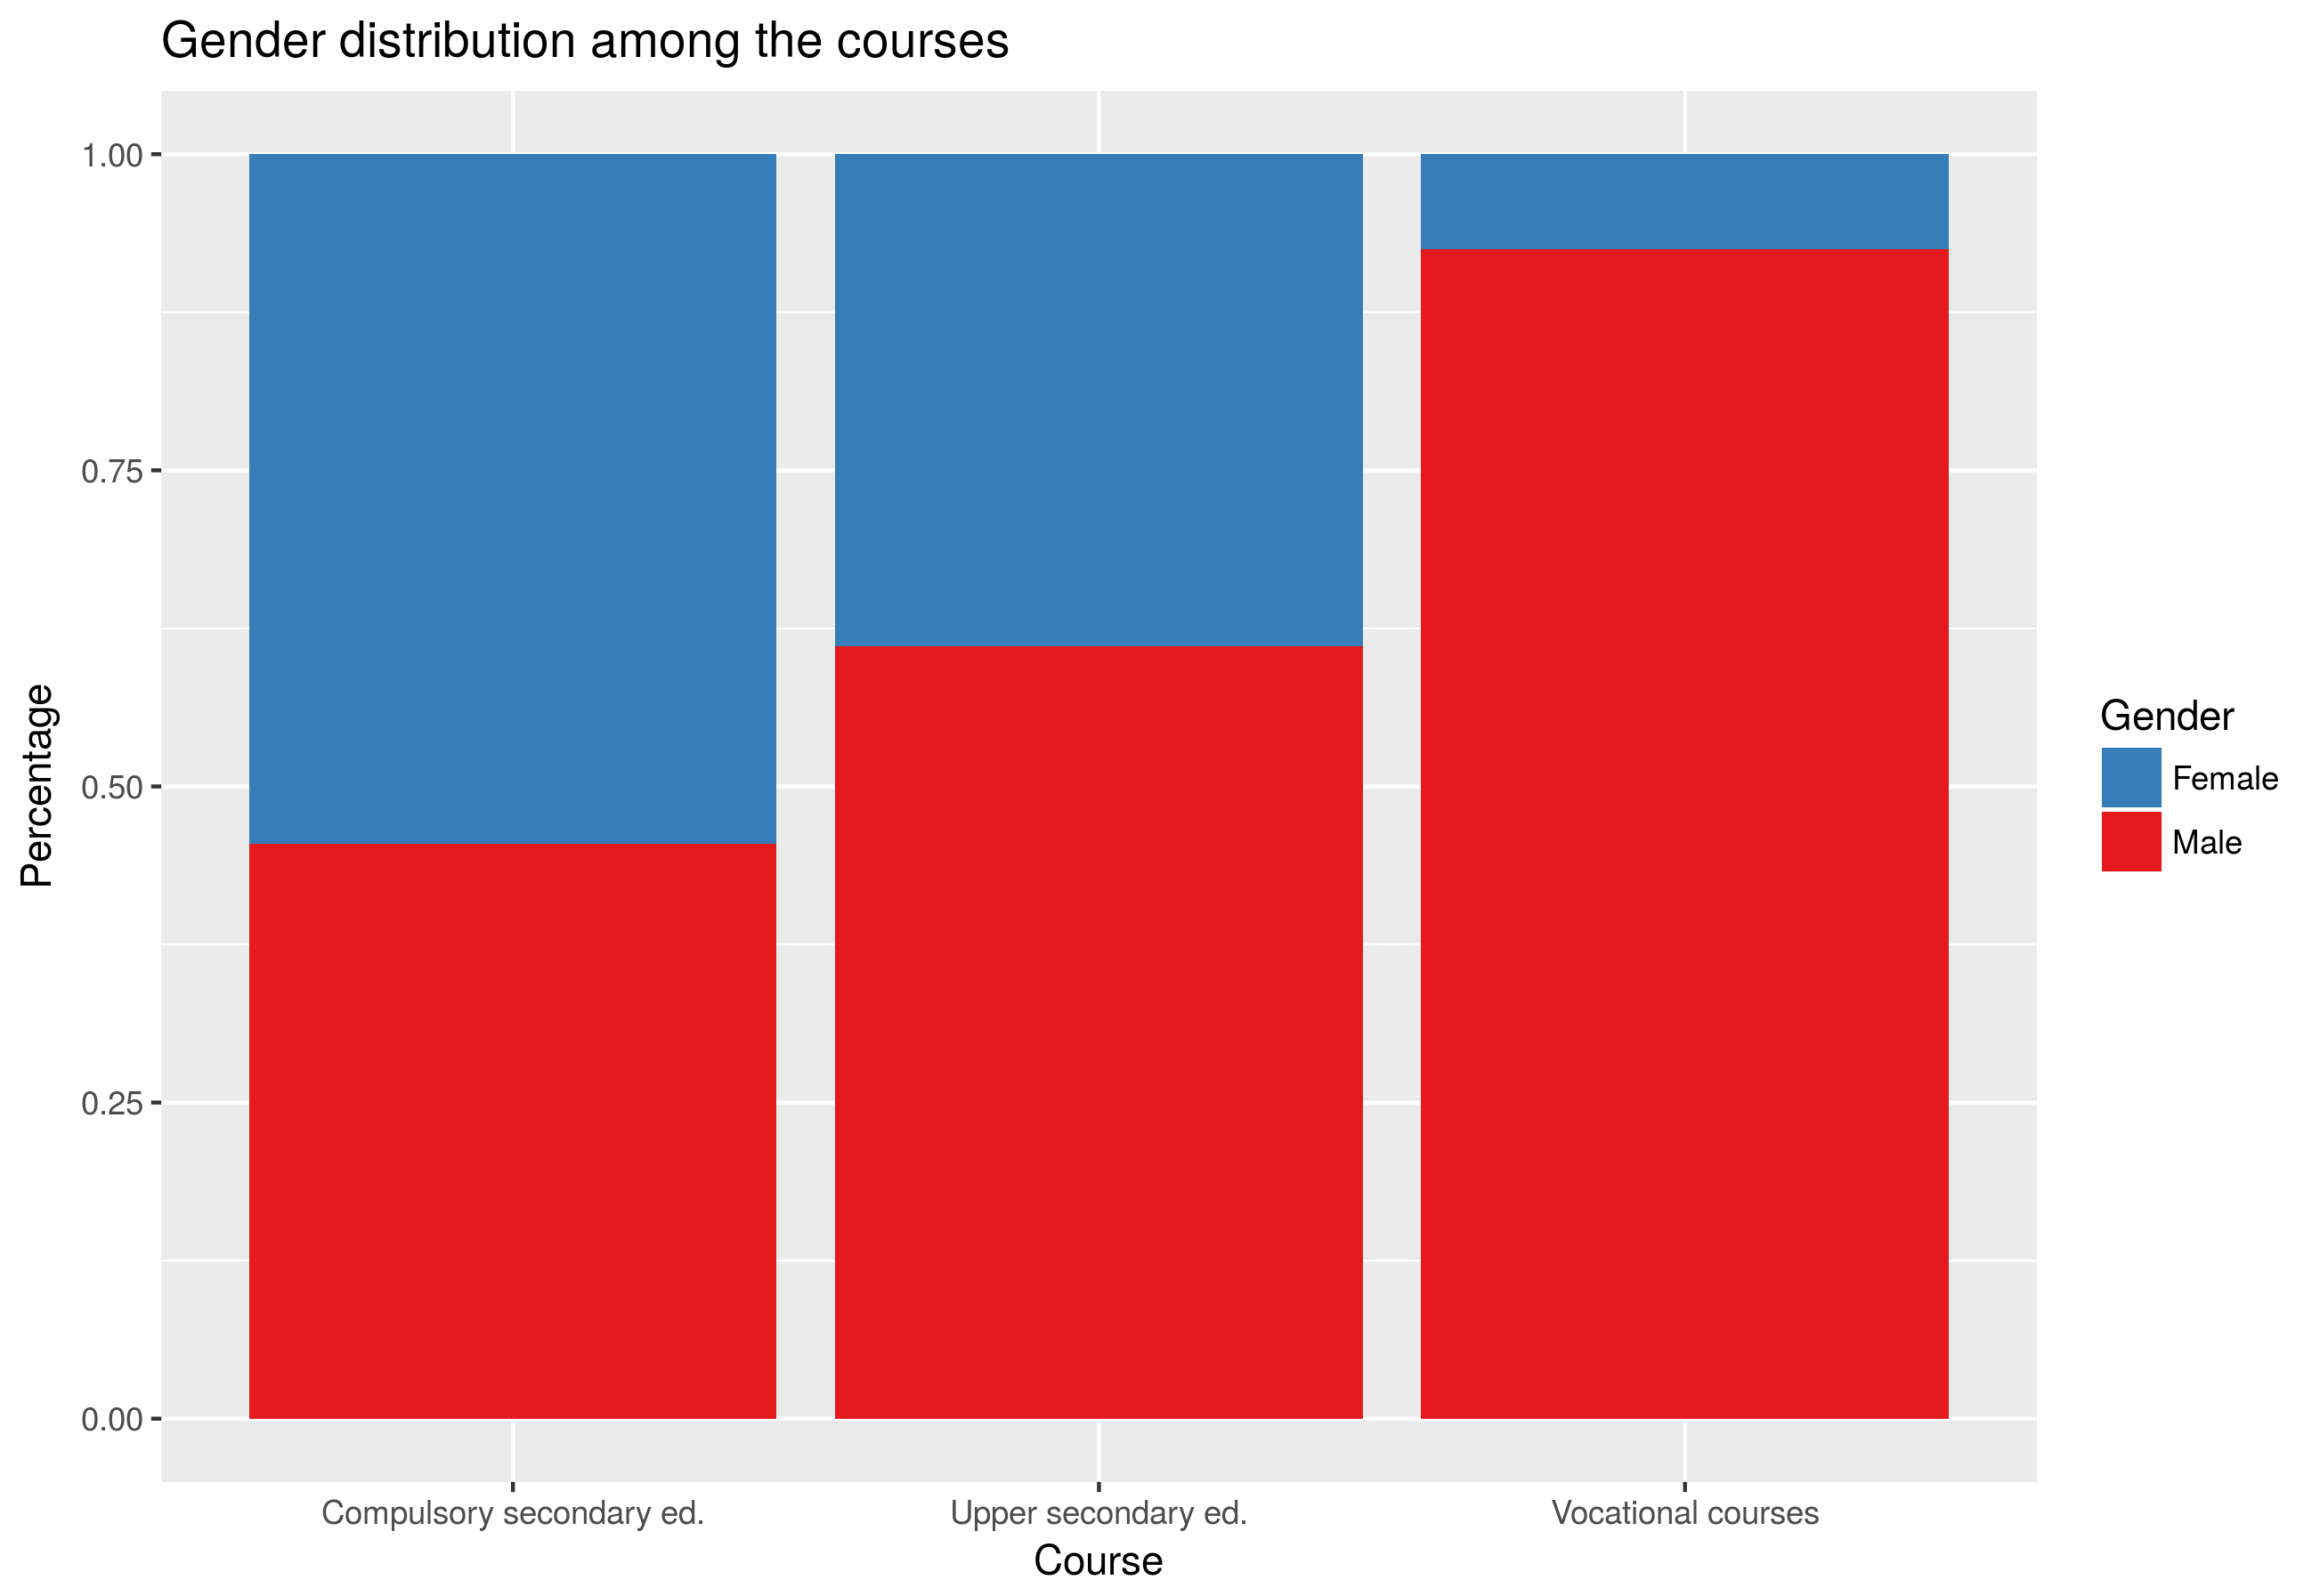
\includegraphics[width=0.5\textwidth]{img/gender_distribution.png}
  \caption{Distribution of gender among the students surveyed, per course. Both academic years 2015-2016 and 2016-2017 are unified.}
  \label{fig:alumni}
\end{figure}

%When asked about their future plans, either if they will continue studying or not, and if the chosen studies will be STEM related, a summary of the responses is depicted in Figure \ref{fig:future}. In this figure, the first two blocks starting from the bottom are immediate higher education in a STEM-related course, and the last one (top of the columns) is the possibility of not studying and look for work instead. It is a logical result that the higher the course is, the most likely is that the students think about working more than to continue studying.
%
%\begin{figure}
%  \centering
%  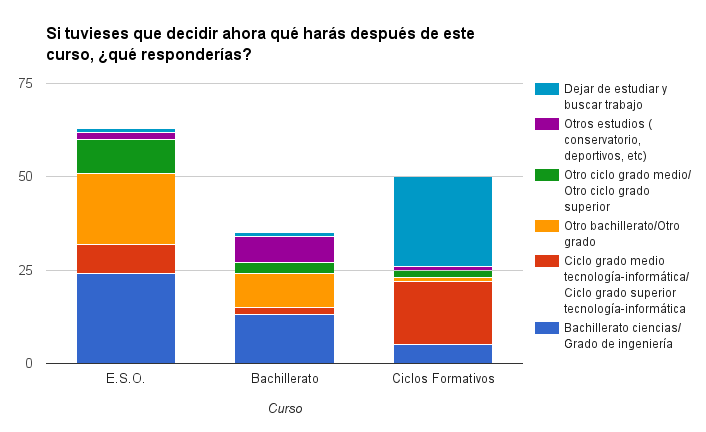
\includegraphics[width=0.5\textwidth]{img/eleccion.png}
%  \caption{Responses to \textit{``If you had to choose right know, what will you do?''} per course. The first two blocks starting from the bottom are immediate higher education in a STEM-related course, and the last one (top of the columns) is the possibility of not studying and look for work instead.}
%  \label{fig:future}
%\end{figure}

Next, we study the opinion of the students about the engineers and the work they perform. To gather their opinions a mutiple choice table was built, presenting a set of statements, to which the students had to mark if they agreed or disagreed (a \textit{``Neutral''} option was also included in case they did not know what to answer). In Figure \ref{fig:opinions} we show a summary of the students' opinions about (from left to right) whether the engineers have a good salary, they have a creative job, their job is easy, has a good work schedule, and their work has an impact on the society. It can be seen that in general, all surveyed students have a good opinion of what an engineer represents to the society and about the possibilities and creativity of their jobs. For the vocational courses, the thought of the engineers having good salaries highly decreases, which may be due to some of the students having already worked in STEM companies and experienced bad conditions. 

\begin{figure}
  \centering
  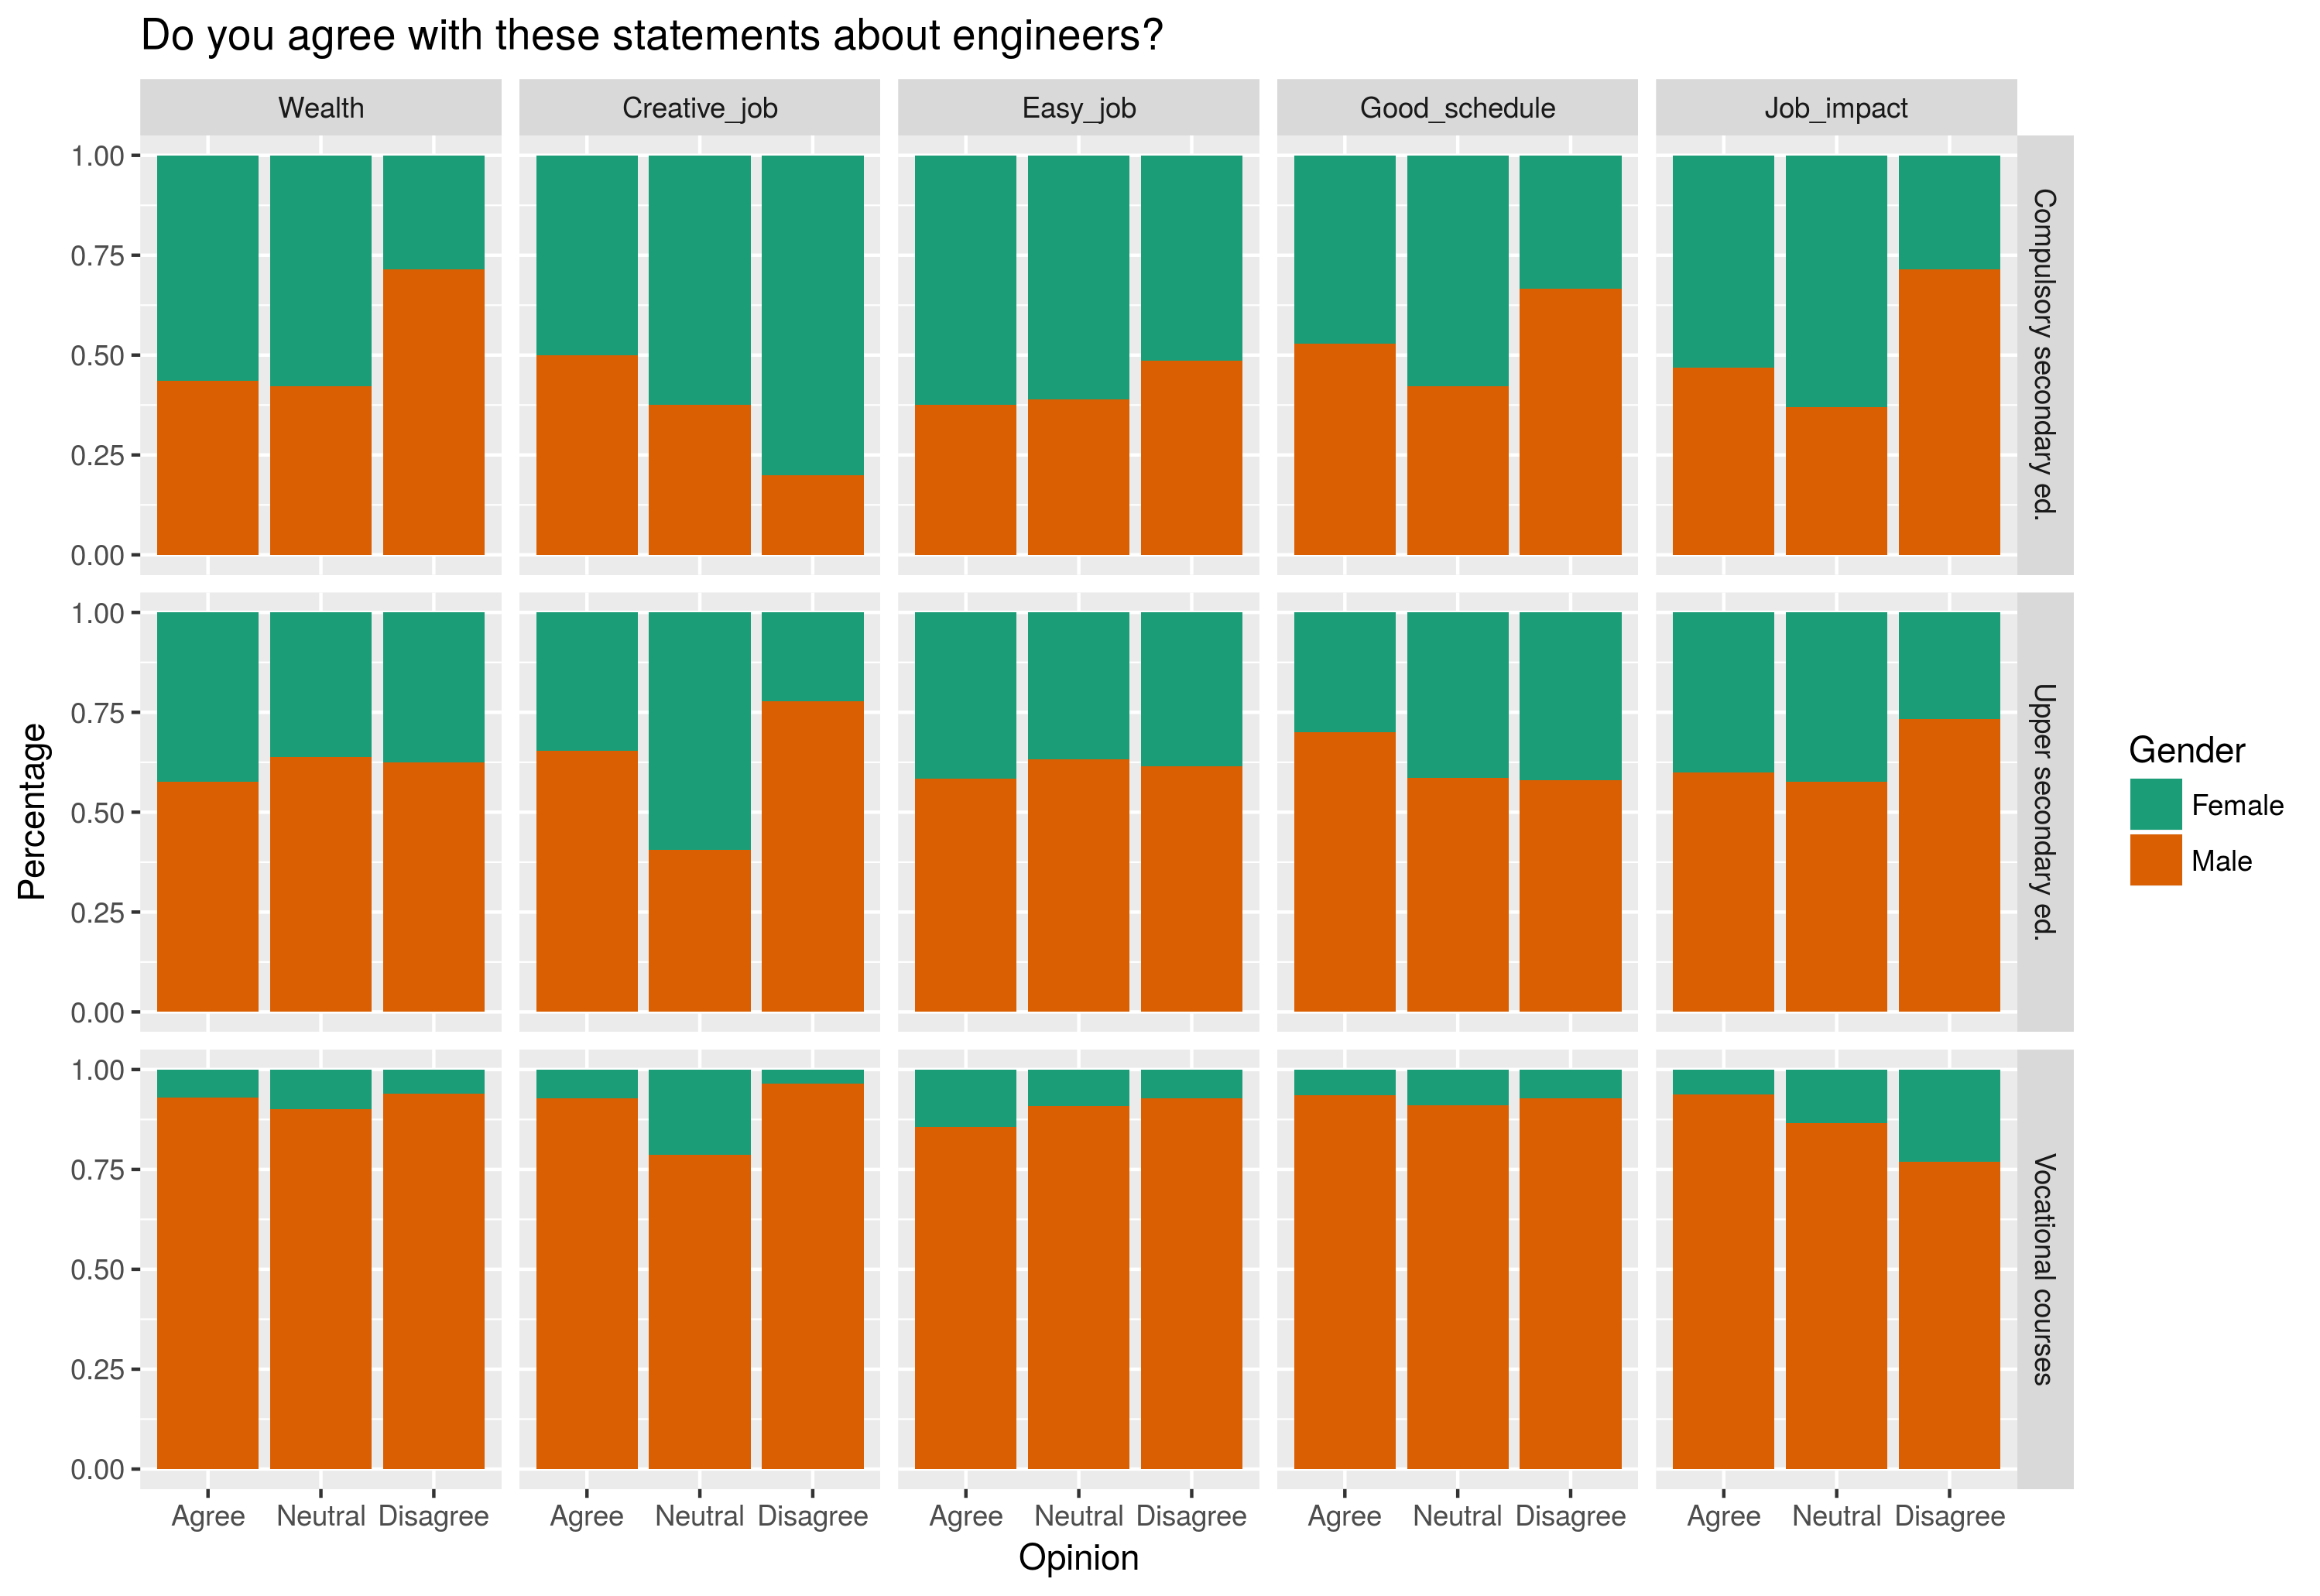
\includegraphics[width=0.5\textwidth]{img/engineer_opinions.png}
  \caption{Responses to different statements made about an engineer per course. Students might agree, disagree, or choose not to give their opinion. Graphics from left to right are related to if the students think that whether an engineer has social prestige, has a good salary, has a creative job, their job is easy, has a good work schedule, and their work has an impact on the society.}
  \label{fig:opinions}
\end{figure}

The same study has been performed with the reasons given by the students when asked why or why not would they study an engineering degree. A list of reasons were provided to the students so that they could explain their feelings about their decision, marking as much reasons as they considered. Figure \ref{fig:opinionsEng} shows a summary of these reasons detailed by course. Graphics from left to right are related to if the students think that: an engineering is good degree choice, in terms of being accesible/easy or having good work opportunities; if they see themselves as capable of study an engineering; if they think it is for men, and if they think it is for `geeks'.

\begin{figure}
	\centering
	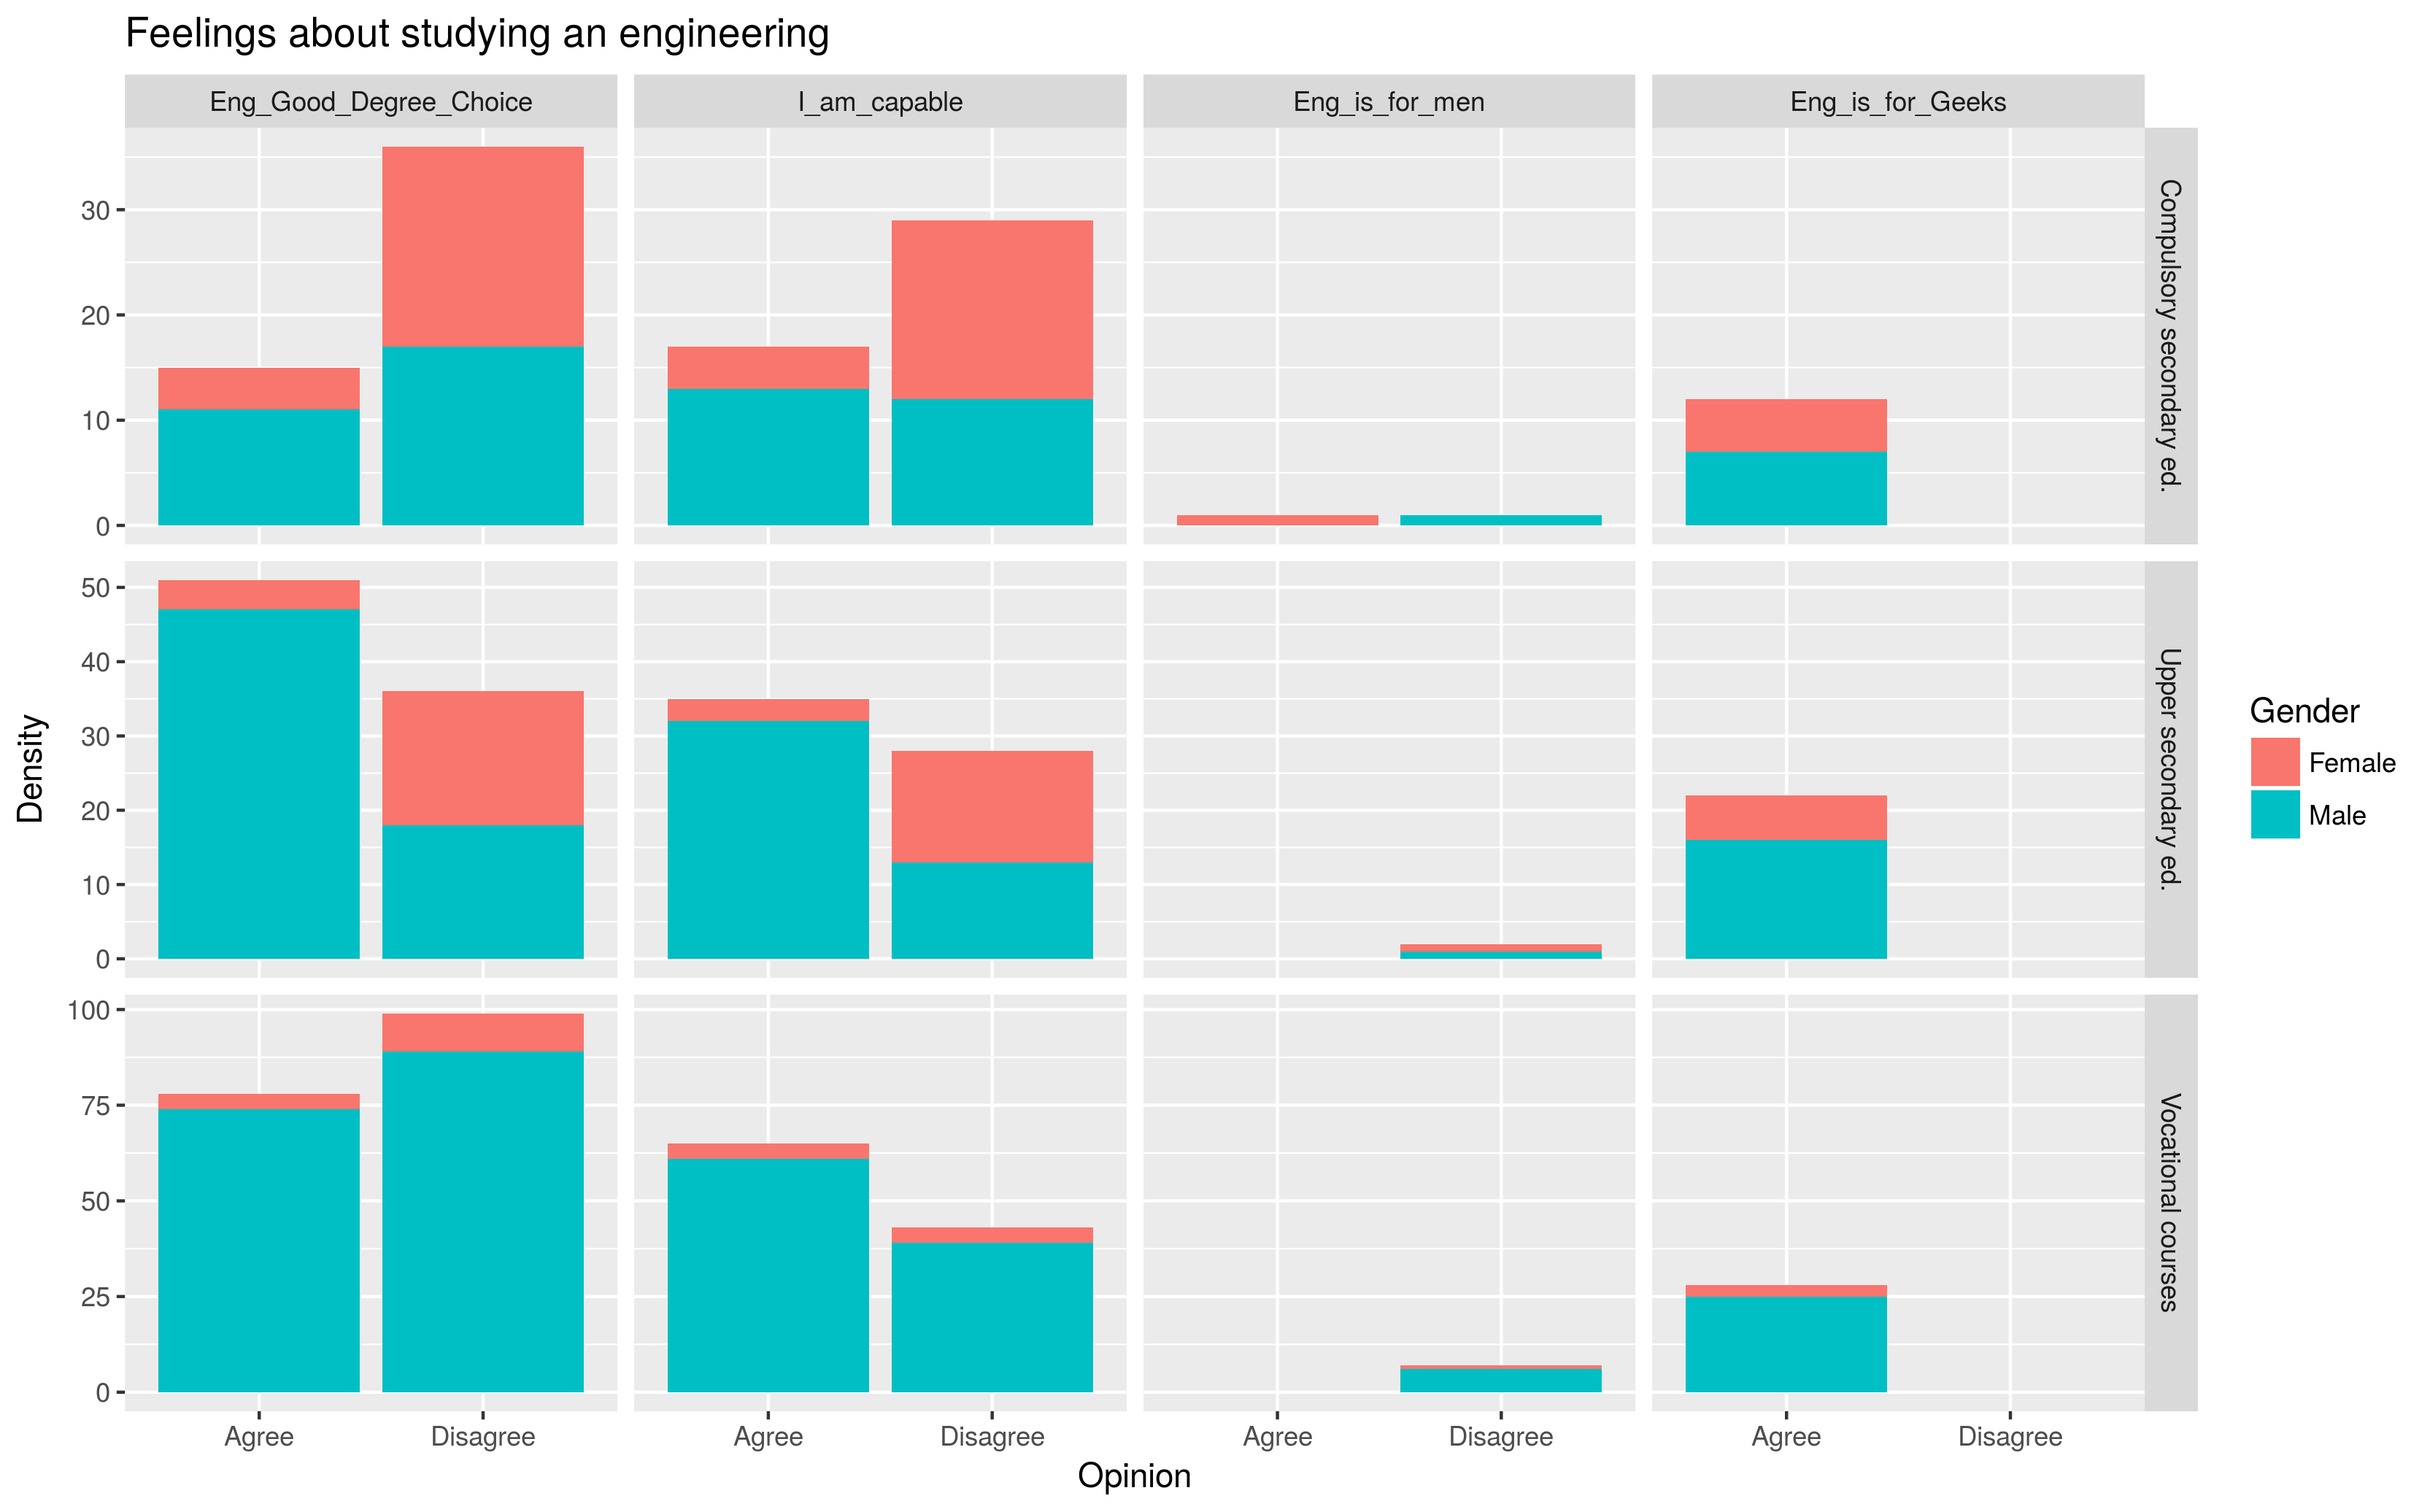
\includegraphics[width=0.5\textwidth]{img/engineering_opinions.png}
	\caption{Reasons given by the students when asked why or why not would they study an engineering degree, detailed by course. Graphics from left to right are related to if the students think that an engineering is good choice for their future, they see themselves as capable of study an engineering, they think it is for men, and for `geeks'.}
	\label{fig:opinionsEng}
\end{figure}

%\begin{table}
%	\caption{{\scriptsize Distribution of surveyed students by academic year.}}
%	\label{tab:muestra}
%	
%	\begin{center}
%		\begin{tabular}{|m{6cm}|c|c|}
%			\hline
%			{\small Academic Year} & {\small Students} & {\small Link to the survey} \\ \hline
%			{\small Tecnología de 3º y 4º de la E.S.O.} & {\small 63} & {\small \url{https://goo.gl/BE3Doa}} \\ \hline
%			{\small Tecnología de 2º de Bachillerato y TIC de 1º de Bachillerato} & {\small 36} & {\small \url{https://goo.gl/usH9Bv}} \\ \hline
%			{\small Ciclos Formativos de Enseñanzas Técnicas} & {\small 50} & {\small \url{https://goo.gl/uDuVxW}} \\ \hline
%		\end{tabular}
%	\end{center}
%\end{table}

\appendix{The Educational System in Spain}
\label{ap:courses}

In order to clarify what students have participated in our study, there is a need for specifying how the educational system works in Spain. High school is divided into 6 years, of which 4 are ``E.S.O.'' (Compulsory secondary education) and ``Bachillerato'' (Upper secondary education). Normally, students from 3rd and 4th courses of E.S.O. and 1st and 2nd courses of Bachillerato range from 15 to 18 years old. There can be students that have repeated a course and be older than 18 years old, but rarely older than 20.

After Bachillerato, students can go to University, work, or study a ``Ciclo Formativo'', which can be understood as a vocational course. They can be accessed from the E.S.O. or from Bachillerato. Thus, depending the course from the courses are accessed, they last four or two years. The vocational courses are organised in a more practical way, and in the case of the study performed for this paper, the students are from:

\begin{itemize}
  \item Network System Administration vocational course
  \item Web applications development vocational course
  \item Multiplatform applications development vocational course
\end{itemize}

All target courses are related to technology or computer science. The students of these courses are not necessary 18 or 19 years old, but sometimes are unnocupied people or University students who had abandoned the degree for a more practical option. 

% An example of a floating figure using the graphicx package.
% Note that \label must occur AFTER (or within) \caption.
% For figures, \caption should occur after the \includegraphics.
% Note that IEEEtran v1.7 and later has special internal code that
% is designed to preserve the operation of \label within \caption
% even when the captionsoff option is in effect. However, because
% of issues like this, it may be the safest practice to put all your
% \label just after \caption rather than within \caption{}.
%
% Reminder: the "draftcls" or "draftclsnofoot", not "draft", class
% option should be used if it is desired that the figures are to be
% displayed while in draft mode.
%
%\begin{figure}[!t]
%\centering
%\includegraphics[width=2.5in]{myfigure}
% where an .eps filename suffix will be assumed under latex, 
% and a .pdf suffix will be assumed for pdflatex; or what has been declared
% via \DeclareGraphicsExtensions.
%\caption{Simulation results for the network.}
%\label{fig_sim}
%\end{figure}

% Note that the IEEE typically puts floats only at the top, even when this
% results in a large percentage of a column being occupied by floats.


% An example of a double column floating figure using two subfigures.
% (The subfig.sty package must be loaded for this to work.)
% The subfigure \label commands are set within each subfloat command,
% and the \label for the overall figure must come after \caption.
% \hfil is used as a separator to get equal spacing.
% Watch out that the combined width of all the subfigures on a 
% line do not exceed the text width or a line break will occur.
%
%\begin{figure*}[!t]
%\centering
%\subfloat[Case I]{\includegraphics[width=2.5in]{box}%
%\label{fig_first_case}}
%\hfil
%\subfloat[Case II]{\includegraphics[width=2.5in]{box}%
%\label{fig_second_case}}
%\caption{Simulation results for the network.}
%\label{fig_sim}
%\end{figure*}
%
% Note that often IEEE papers with subfigures do not employ subfigure
% captions (using the optional argument to \subfloat[]), but instead will
% reference/describe all of them (a), (b), etc., within the main caption.
% Be aware that for subfig.sty to generate the (a), (b), etc., subfigure
% labels, the optional argument to \subfloat must be present. If a
% subcaption is not desired, just leave its contents blank,
% e.g., \subfloat[].


% An example of a floating table. Note that, for IEEE style tables, the
% \caption command should come BEFORE the table and, given that table
% captions serve much like titles, are usually capitalized except for words
% such as a, an, and, as, at, but, by, for, in, nor, of, on, or, the, to
% and up, which are usually not capitalized unless they are the first or
% last word of the caption. Table text will default to \footnotesize as
% the IEEE normally uses this smaller font for tables.
% The \label must come after \caption as always.
%
%\begin{table}[!t]
%% increase table row spacing, adjust to taste
%\renewcommand{\arraystretch}{1.3}
% if using array.sty, it might be a good idea to tweak the value of
% \extrarowheight as needed to properly center the text within the cells
%\caption{An Example of a Table}
%\label{table_example}
%\centering
%% Some packages, such as MDW tools, offer better commands for making tables
%% than the plain LaTeX2e tabular which is used here.
%\begin{tabular}{|c||c|}
%\hline
%One & Two\\
%\hline
%Three & Four\\
%\hline
%\end{tabular}
%\end{table}


% Note that the IEEE does not put floats in the very first column
% - or typically anywhere on the first page for that matter. Also,
% in-text middle ("here") positioning is typically not used, but it
% is allowed and encouraged for Computer Society conferences (but
% not Computer Society journals). Most IEEE journals/conferences use
% top floats exclusively. 
% Note that, LaTeX2e, unlike IEEE journals/conferences, places
% footnotes above bottom floats. This can be corrected via the
% \fnbelowfloat command of the stfloats package.




\section{Conclusion}
The conclusion goes here.





% if have a single appendix:
%\appendix[Proof of the Zonklar Equations]
% or
%\appendix  % for no appendix heading
% do not use \section anymore after \appendix, only \section*
% is possibly needed

% use appendices with more than one appendix
% then use \section to start each appendix
% you must declare a \section before using any
% \subsection or using \label (\appendices by itself
% starts a section numbered zero.)
%


%\appendices
%\section{Proof of the First Zonklar Equation}
%Appendix one text goes here.

% you can choose not to have a title for an appendix
% if you want by leaving the argument blank
%\section{}
%Appendix two text goes here.


% use section* for acknowledgment
\section*{Acknowledgment}

The authors would like to thank to the high school ``Zaid\'{i}n-Vergeles'' for their collaboration during the performance of the surveys.


% Can use something like this to put references on a page
% by themselves when using endfloat and the captionsoff option.
\ifCLASSOPTIONcaptionsoff
  \newpage
\fi



% trigger a \newpage just before the given reference
% number - used to balance the columns on the last page
% adjust value as needed - may need to be readjusted if
% the document is modified later
%\IEEEtriggeratref{8}
% The "triggered" command can be changed if desired:
%\IEEEtriggercmd{\enlargethispage{-5in}}

% references section

% can use a bibliography generated by BibTeX as a .bbl file
% BibTeX documentation can be easily obtained at:
% http://mirror.ctan.org/biblio/bibtex/contrib/doc/
% The IEEEtran BibTeX style support page is at:
% http://www.michaelshell.org/tex/ieeetran/bibtex/
%\bibliographystyle{IEEEtran}
% argument is your BibTeX string definitions and bibliography database(s)
%\bibliography{IEEEabrv,../bib/paper}
%
% <OR> manually copy in the resultant .bbl file
% set second argument of \begin to the number of references
% (used to reserve space for the reference number labels box)
\bibliographystyle{IEEEtran}
\bibliography{genderEngineering}

% biography section
% 
% If you have an EPS/PDF photo (graphicx package needed) extra braces are
% needed around the contents of the optional argument to biography to prevent
% the LaTeX parser from getting confused when it sees the complicated
% \includegraphics command within an optional argument. (You could create
% your own custom macro containing the \includegraphics command to make things
% simpler here.)
%\begin{IEEEbiography}[{\includegraphics[width=1in,height=1.25in,clip,keepaspectratio]{mshell}}]{Michael Shell}
% or if you just want to reserve a space for a photo:

\begin{IEEEbiographynophoto}{Paloma de las Cuevas}
Biography text here.
\end{IEEEbiographynophoto}

% if you will not have a photo at all:
\begin{IEEEbiographynophoto}{Maribel Garc\'{i}a-Arenas}
Biography text here.
\end{IEEEbiographynophoto}

% insert where needed to balance the two columns on the last page with
% biographies
%\newpage

%\begin{IEEEbiographynophoto}{Jane Doe}
%Biography text here.
%\end{IEEEbiographynophoto}

% You can push biographies down or up by placing
% a \vfill before or after them. The appropriate
% use of \vfill depends on what kind of text is
% on the last page and whether or not the columns
% are being equalized.

%\vfill

% Can be used to pull up biographies so that the bottom of the last one
% is flush with the other column.
%\enlargethispage{-5in}

% that's all folks
\end{document}
